\section{Module hồi quy tư thế tương đối - RPR}
Mô hình tương quan 2D-2D được đề xuất trong Map-free Relocalization \cite{arnold2022mapfree} thuộc nhóm những phương pháp định vị theo hướng tiếp cận truyền thống sử dụng Essential Matrix. So với những phương pháp RPR thường thấy, phương pháp này giải quyết được vấn đề không nắm bắt được thông tin về hình học trong ảnh. Mô hình vẫn đạt được kết quả cạnh tranh trong những môi trường có mật độ ảnh dày đặc. Tuy nhiên, khi được đưa vào môi trường mà ảnh tham khảo và ảnh truy vấn xa nhau hơn thì phương pháp này lại có kết quả vượt trội hơn hẳn những phương pháp khác. Mô hình tương quan 2D-2D xác định Essential Matrix giữa 2 ảnh thông qua những cặp điểm tương quan, từ đó tính toán được khác biệt về hướng lệch vị trí và góc quay. Sử dụng thêm thông tin về độ sâu, mô hình xác định được khoảng cách cách biệt thực giữa cặp ảnh và qua đó có được vị trí thực của ảnh truy vấn.

\subsection{Kiến trúc}

\begin{figure}[htbp]
  \centering
  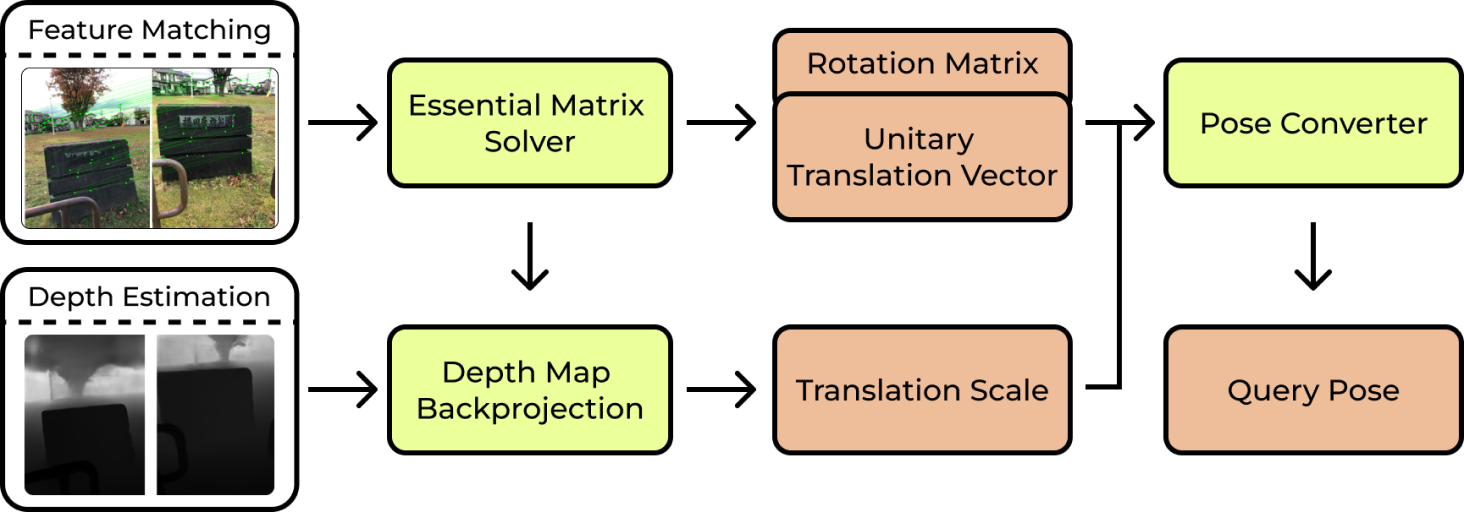
\includegraphics[width=\textwidth]{pics/Proposal/2d_2d.png}
  % \includesvg[scale=0.3]{pics/Proposal/arch.svg}
  \caption{Kiến trúc tổng quan của mô hình tương quan 2D-2D}
\end{figure}

\subsubsection{Mô hình xác định cặp đặc trưng và ước tính độ sâu của ảnh}

Với dữ liệu đầu vào là cặp ảnh gồm ảnh truy vấn và ảnh tham khảo $(I, I_0)$, tại bước này, những cặp đặc trưng tương quan sẽ được xác định và vị trí của chúng sẽ được lưu lại trong 2 tập là $(kpts_0, ktps_1)$. Mô hình ghép đặc trưng được sử dụng sẽ là SuperPoint+SuperGlue \cite{sarlin2020superglue} đã trải qua quá trình huấn luyện. Bản đồ thông tin độ sâu của mỗi ảnh cũng sẽ được sinh ra bằng mô hình DPT \cite{ranftl2021vision} được huấn luyện trên tập KITTI do phạm vi được sử dụng của mô hình sẽ là ở ngoài trời, trong khu vực thành thị \cite{arnold2022mapfree}. Dữ liệu trả về của 2 mô hình này sẽ là hai tập chứa vị trí của các điểm đặc trưng tương ứng và bản đồ độ sâu ước tính của mỗi hình.

\begin{figure}[H]
  \centering
  \begin{minipage}[b]{0.48\textwidth}
    \captionsetup{justification=centering}
    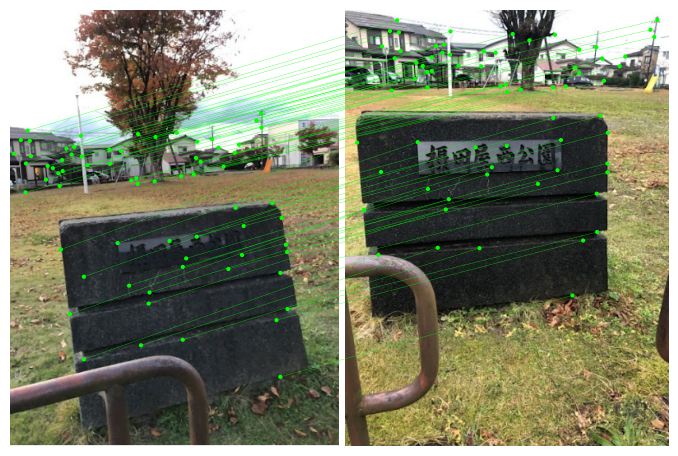
\includegraphics[width=\textwidth]{pics/Proposal/matching.png}
    \caption{Kết quả của quá trình xác định và ghép đặc trưng}
  \end{minipage}
  \begin{minipage}[b]{0.48\textwidth}
    \captionsetup{justification=centering}
    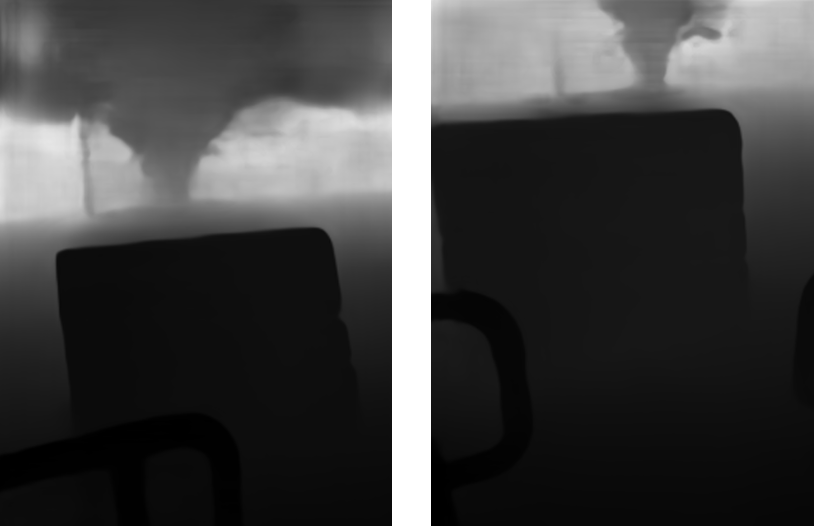
\includegraphics[width=\textwidth]{pics/Proposal/depth.png}
    \caption{Kết quả của quá trình ước tính độ sâu ảnh}
  \end{minipage}
  % \begin{minipage}[t]{0.3\textwidth}
  %     \caption{Kết quả của quá trình xác định và ghép đặc trưng}
  % \end{minipage}
  % \begin{minipage}[t]{0.3\textwidth}
  %     \caption{Kết quả của quá trình ước tính độ sâu ảnh}
  % \end{minipage}
\end{figure}

\subsubsection{Bộ phận khai phá Essential Matrix}

Dựa vào những cặp đặc trưng tương quan đã được xác định trong các tập $(kpts_0, kpts_1)$ và ma trận thông số $T_0, T_1$ của camera của mỗi ảnh, Essential Matrix $M$ được ước tính dựa vào giải thuật 5 điểm \cite{nister2004efficient} cùng với vòng lặp MAGSAC++ \cite{barath2020magsac++}. Ma trận thông số $T_i$ của camera sẽ chứa các thông tin về tiêu cự của camera $f_x,f_y$ và tọa độ điểm chính của camera $c_x,c_y$, được sắp xếp thành ma trận như sau:
\begin{equation}
  T_i = \begin{bmatrix} f_x & 0 & c_x \\ 0 & f_y & c_y \\ 0 & 0 & 1 \end{bmatrix}
\end{equation}
Essential Matrix $M$ sau đó sẽ được phân giải thành ma trận thể hiện góc quay chênh lệch, $R \in SO(3)$ và vector đơn vị độ lệch về vị trí giữa hai ảnh, $\hat{t} \in R^{3}, \lvert \hat{t} \rvert = 1$. Tập những cặp điểm tương quan thỏa Essential Matrix $M$ cũng sẽ được trả về.

\subsubsection{Bộ phận chiếu cặp điểm tương quan lên không gian ba chiều}

Những cặp điểm tương quan (inlier correspondence) thỏa ma trận $M$ sau đó sẽ được chiếu lên không gian 3D qua bản đồ độ sâu ảnh đã được sinh ra ở mỗi ảnh. Với mỗi cặp điểm $p_0, p_1$ đã được chiếu lên không gian 3D, mô hình sẽ tìm được một giá trị tỷ lệ $s^*$ cho $\hat{t}$ để làm giảm thiểu độ lệch của điểm $p_0$ khi được chiếu lên hệ tọa độ của camera thứ hai và điểm $p_1$. Giá trị $s$ tương ứng với mỗi cặp điểm $(p_0, p_1)$ có thể được xác định qua công thức:

\begin{equation}
  \begin{aligned}
    s=\underset{s^*}{\arg \min }\left\|R p_A+s^* \cdot \hat{t}-p_B\right\|_2 .
  \end{aligned}
\end{equation}

\begin{figure}[H]
  \centering
  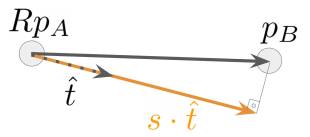
\includegraphics[scale=1]{pics/Proposal/reprojection.png}
  \caption[Minh họa cho việc xác định tỷ lệ $s$ bằng độ sâu ảnh]{Hình minh họa cho việc chiếu điểm $p_0$ qua vector góc quay $R$ và vector độ lệch đơn vị $\hat{t}$ cùng với tỷ lệ $s$ để tối thiểu khoảng cách \cite{arnold2022mapfree}}
\end{figure}

Cuối cùng, tỷ lệ $s^*$ với số cặp điểm hợp lệ cao nhất sẽ được chọn làm kết quả cuối cùng. Một cặp điểm sẽ được xem như hợp lệ khi khoảng cách sai lệch giữa hai điểm 3D sau khi chiếu nhỏ hơn một ngưỡng nhất định, ở đây được xác định là 10cm. Vòng lặp RANSAC sẽ được sử dụng để bỏ những trường hợp ngoại lệ.

Sau khi chạy qua những bước trên, mô hình sẽ thu về được các giá trị thể hiện độ lệch giữa vị trí và góc quay của cặp ảnh truy vấn và tham khảo dưới dạng ma trận độ lệch góc quay $R$ và vector độ lệch vị trí $s*\hat{t}$. Ma trận độ lệch góc quay $R$ sau đó sẽ được phân giải thành một Quaternion - được biểu diễn dưới dạng một tập 4 số là $q^{\Delta} = (q^{\Delta}_w,q^{\Delta}_x,q^{\Delta}_y,q^{\Delta}_z)$ - thể hiện góc quay trong không gian. Vector độ lệch vị trí sẽ có dạng bộ 3 số là $(t^{\Delta} = t^{\Delta}_x,t^{\Delta}_y,t^{\Delta}_z)$. Ngoài ra, số cặp điểm tương quan có độ lệch dưới 10cm với giá trị $s^*$ được chọn sẽ được dùng làm thông số đánh giá độ đáng tin cậy $C$ của dự đoán.


\subsubsection{Bộ phận tính toán tư thế tuyệt đối}

Từ kết quả của những bộ phận trên, mô hình đã biểu diễn được góc quay và vị trí tương đối giữa hai ảnh $(q^{\Delta},t^{\Delta})$. Khi biết được tọa độ chính xác của ảnh tham khảo $(q^{ref},t^{ref})$, mô hình sẽ tính được tọa độ và góc quay chính xác của ảnh truy vấn và đưa ra kết quả cuối cùng là hai tập $(q^{abs},t^{abs})$

Để xác định được góc quay chính xác của ảnh truy vấn, mô hình biến đổi góc quay của ảnh tham khảo với độ lệch góc quay đã xác định được giữa hai ảnh theo công thức:

\begin{equation}
  \begin{aligned}
    q^{abs}                                   & = q^{\Delta} * q^{ref}                                                                                    \\
    (q^{abs}_w,q^{abs}_x,q^{abs}_y,q^{abs}_z) & = (q^{\Delta}_w,q^{\Delta}_x,q^{\Delta}_y,q^{\Delta}_z) * (q^{ref}_w,q^{ref}_x,q^{ref}_y,q^{ref}_z)       \\ \\
    q^{abs}_w                                 & =\left(q^{\Delta}_w q^{ref}_w-q^{\Delta}_x q^{ref}_x-q^{\Delta}_y q^{ref}_y-q^{\Delta}_z q^{ref}_z\right) \\
    q^{abs}_x                                 & =\left(q^{\Delta}_w q^{ref}_x+q^{\Delta}_x q^{ref}_w-q^{\Delta}_y q^{ref}_z+q^{\Delta}_z q^{ref}_y\right) \\
    q^{abs}_y                                 & =\left(q^{\Delta}_w q^{ref}_y+q^{\Delta}_x q^{ref}_z+q^{\Delta}_y q^{ref}_w-q^{\Delta}_z q^{ref}_x\right) \\
    q^{abs}_z                                 & =\left(q^{\Delta}_w q^{ref}_z-q^{\Delta}_x q^{ref}_y+q^{\Delta}_y q^{ref}_x+q^{\Delta}_z q^{ref}_w\right)
  \end{aligned}
\end{equation}

Để xác định vị trí chính xác của ảnh truy vấn trong không gian thực, vị trí kinh độ, vĩ độ và độ cao của ảnh chụp có thể được xác định qua công thức:

\begin{equation}
  \begin{aligned}
    t^{abs}                         & = t^{\Delta} + t^{ref}                                                       \\
    (t^{abs}_x,t^{abs}_y,t^{abs}_z) & = (t^{\Delta}_x,t^{\Delta}_y,t^{\Delta}_z) + (t^{ref}_x,t^{ref}_y,t^{ref}_z) \\ \\
    t^{abs}_x                       & = t^{\Delta}_x + t^{ref}_x                                                   \\
    t^{abs}_y                       & = t^{\Delta}_y + t^{ref}_y                                                   \\
    t^{abs}_z                       & = t^{\Delta}_z + t^{ref}_z                                                   \\
  \end{aligned}
\end{equation}

\subsection{Phương pháp hiện thực và triển khai}
\subsubsection{Hiện thực}
Tác vụ tìm kiếm tương quan giữa hai ảnh có thể lựa chọn giữa các phương pháp truyền thống như SIFT, hoặc những phương pháp theo hướng tiếp cận học sâu gần đây như SuperPoint+SuperGlue \cite{sarlin2020superglue} và LoFTR \cite{sun2021loftr}. Tác vụ tính độ sâu đơn ảnh sẽ được phân thành hai trường hợp là bên trong nhà và ngoài trời. Với những tập dữ liệu trong nhà, mô hình DPT \cite{ranftl2021vision} được huấn luyện trên tập dữ liệu NYUv2 \cite{silberman2012indoor} PlaneRCNN \cite{liu2019planercnn} được huấn luyện trên tập dữ liệu ScanNet \cite{dai2017scannet}. Với trường hợp ngoài trời, mô hình DPT \cite{ranftl2021vision} được huấn luyện trên tập KITTI sẽ được sử dụng \cite{geiger2012we}. Mô hình SuperPoint+SuperGlue sẽ được chọn để thực hiện tác vụ Feature Matching và mô hình DPT được huấn luyện trên tập KITTI sẽ được dùng để thực hiện tác vụ Monocular Depth Estimation, nhờ vào độ chính xác cao thể hiện trong \cite{arnold2022mapfree}.

\subsubsection{Phương pháp đánh giá}
Để đánh giá hiệu quả của mô hình trong tác vụ định vị trực quan, một số tiêu chí cơ bản đã được đưa ra như độ lệch về góc quay, độ lệch về vị trí của camera, cũng như một sai số mới được đưa ra trong bài nghiên cứu, sai số phản chiếu của điểm 3D ảo - VCRE, được lấy cảm hứng từ sai số phản chiếu của những điểm tương ứng - DCRE \cite{wald2020beyond}. Cụ thể, với giá trị dự đoán $(R,t)$ và giá trị thực $(R_{gt},t_{gt})$, các sai số sẽ được xác định như sau:
\begin{itemize}
  \item Sai số về góc quay, $\measuredangle(R,R_{gt})$, sẽ được tính là độ chênh lệch giữa góc quay được dự đoán và góc quay thực tế.
  \item Sai số về độ lệch vị trí máy quay sẽ được tính là khoảng cách Euclidean giữa cặp vị trí $(t,t_{gt})$ được tính theo công thức $c=-R \intercal t$.
  \item Sai số phản chiếu của điểm 3D ảo sẽ được dùng để đánh giá độ lệch của những vật thể trong không gian thực tế ảo. Giá trị thực $(R_{gt},t_{gt})$ và giá trị dự đoán $(R,t)$ sẽ được dùng để chiếu những điểm 3D ảo, lên hệ tọa độ của camera truy vấn. Giá trị VCRE sẽ được xác định theo công thức
        \begin{equation}
          \operatorname{VCRE}=\frac{1}{|\mathcal{V}|} \sum_{\mathbf{v} \in \mathcal{V}}\left\|\pi(\mathbf{v})-\pi\left(T T_{\mathrm{gt}}^{-1} \mathbf{v}\right)\right\|_2 \quad \text { với } T=[R \mid t]
        \end{equation}

        với $\pi$ là phép chiếu từ không gian camera lên ảnh, $\mathcal{V}$ là một tập các điểm 3D, đại diện cho những vật thể ảo. $\mathcal{V}$ là một lưới điểm 3D, (chiều cao là 4, chiều rộng là 7 và chiều sâu là 7), cách nhau 30cm và có độ dịch là 1.8m dọc theo trục của máy ảnh. Giá trị sai số của phép phản chiếu sẽ được so sánh với đường chéo của ảnh.
  \item Độ tin cậy $C$ của dự đoán cũng là một tiêu chí được đánh giá. Giá trị này cho phép mô hình có thể phát hiện và loại bỏ những dự đoán không đáng tin cậy. Giá trị này sẽ được xác định bằng số lượng cặp điểm tương quan thỏa Essential Matrix được chọn trên tổng số cặp điểm tương quan xác định bởi mô hình ghép đặc trưng. Với một ngưỡng tin cậy nhất định, tỷ lệ dự đoán đáng tin cậy - ratio of confident estimate, sẽ được xác định là tỷ lệ ảnh truy vấn có độ tin cậy vượt qua ngưỡng.
  \item Độ chính xác của mô hình sẽ là tỷ lệ ảnh đáng tin cậy có sai lệch giữa giá trị dự đoán và giá trị thực dưới một ngưỡng nhất định (độ lệch vị trí và góc quay) hoặc có sai số phản chiếu chấp nhận được trên tổng số ảnh.
\end{itemize}

Tập dữ liệu 7Scenes \cite{6619221} được sử dụng để xác định hiệu suất mô hình tiêu chuẩn của Map-free so với những phương pháp SOTA tại thời điểm đó, với số lượng ảnh tham khảo là rất nhiều. Ảnh hưởng của việc giảm số lượng ảnh tham khảo lên khả năng hoạt động của các mô hình cũng sẽ được ghi nhận lại. Tập dữ liệu Niantic \cite{arnold2022mapfree} được đề xuất trong cùng bài nghiên cứu cũng sẽ được sử dụng để đánh giá, nhằm xác định hiệu suất của các mô hình trong trường hợp chỉ có một ảnh tham khảo.


\subsection{Kết quả}
\subsubsection{Tập dữ liệu 7Scenes}

\begin{table}[H]
  \adjustbox{max width=\textwidth}{
    \begin{tabular}{|c|r|c|c|}
      \hline
      \multicolumn{1}{|l|}{\textbf{}}                                                                  & \textbf{Method}                                                                      & \textbf{\begin{tabular}[c]{@{}c@{}}Average Median\\ Pose Error\end{tabular}} & \textbf{\begin{tabular}[c]{@{}c@{}}Precision @ VCRE\\ 5\% / 10\% diag\end{tabular}} \\ \hline
                                                                                                       & \cellcolor[HTML]{C5FFD9}DSAC*                                                        & \cellcolor[HTML]{C5FFD9}3 cm, 1.1°                                           & \cellcolor[HTML]{C5FFD9}0.98/0.99                                                   \\
                                                                                                       & \cellcolor[HTML]{C5FFD9}hLoc                                                         & \cellcolor[HTML]{C5FFD9}3 cm, 1.0°                                           & \cellcolor[HTML]{C5FFD9}N/A                                                         \\
      \multirow{-3}{*}{\textbf{\begin{tabular}[c]{@{}c@{}}Structure\\ -based\end{tabular}}}            & \cellcolor[HTML]{C5FFD9}ActiveSearch                                                 & \cellcolor[HTML]{C5FFD9}4 cm, 1.2°                                           & \cellcolor[HTML]{C5FFD9}N/A                                                         \\ \hline
                                                                                                       & \cellcolor[HTML]{C5FFD9}EssNet (Ess.Mat.)                                            & \cellcolor[HTML]{C5FFD9}22 cm, 8.0°                                          & \cellcolor[HTML]{C5FFD9}N/A                                                         \\
                                                                                                       & \cellcolor[HTML]{F8BA5D}ExReNet                                                      & \cellcolor[HTML]{F8BA5D}9 cm, 2.7°                                           & \cellcolor[HTML]{F8BA5D}N/A                                                         \\
                                                                                                       & \cellcolor[HTML]{ECF4FF}ExReNet                                                      & \cellcolor[HTML]{ECF4FF}12 cm, 3.3°                                          & \cellcolor[HTML]{ECF4FF}N/A                                                         \\
                                                                                                       & \cellcolor[HTML]{ECF4FF}SIFT (Ess.Mat.)                                              & \cellcolor[HTML]{ECF4FF}8 cm, 2.0°                                           & \cellcolor[HTML]{ECF4FF}0.87/0.93                                                   \\
      \multirow{-5}{*}{\textbf{\begin{tabular}[c]{@{}c@{}}Pose\\ Triangulation\end{tabular}}}          & \cellcolor[HTML]{ECF4FF}SuperGlue (Ess.Mat.)                                         & \cellcolor[HTML]{ECF4FF}7 cm, 1.5°                                           & \cellcolor[HTML]{ECF4FF}0.93/0.97                                                   \\ \hline
                                                                                                       & \cellcolor[HTML]{ECF4FF}RelocNet                                                     & \cellcolor[HTML]{ECF4FF}29 cm, 11.3°                                         & \cellcolor[HTML]{ECF4FF}N/A                                                         \\
                                                                                                       & \cellcolor[HTML]{ECF4FF}RPR {[}R($\alpha$,$\beta$,$\gamma$)+s.t($\theta$, $\phi$){]} & \cellcolor[HTML]{ECF4FF}18 cm, 4.9°                                          & \cellcolor[HTML]{ECF4FF}0.71/0.93                                                   \\
      \multirow{-3}{*}{\textbf{RPR}}                                                                   & \cellcolor[HTML]{ECF4FF}RPR {[}3D-3D{]}                                              & \cellcolor[HTML]{ECF4FF}16 cm, 4.5°                                          & \cellcolor[HTML]{ECF4FF}0.82/0.96                                                   \\ \hline
                                                                                                       & \cellcolor[HTML]{ECF4FF}SIFT (Ess.Mat.+D.Scale)                                      & \cellcolor[HTML]{ECF4FF}16 cm, 2.5°                                          & \cellcolor[HTML]{ECF4FF}0.84/0.94                                                   \\
                                                                                                       & \cellcolor[HTML]{ECF4FF}SuperGlue (Ess.Mat.+D.Scale)                                 & \cellcolor[HTML]{ECF4FF}13 cm, 1.8°                                          & \cellcolor[HTML]{ECF4FF}0.89/0.97                                                   \\
                                                                                                       & \cellcolor[HTML]{ECF4FF}SIFT (PnP)                                                   & \cellcolor[HTML]{ECF4FF}12 cm, 3.3°                                          & \cellcolor[HTML]{ECF4FF}0.89/0.95                                                   \\
      \multirow{-4}{*}{\textbf{\begin{tabular}[c]{@{}c@{}}Feat.matching\\ + Depth Scale\end{tabular}}} & \cellcolor[HTML]{ECF4FF}SuperGlue (PnP)                                              & \cellcolor[HTML]{ECF4FF}10 cm, 2.8°                                          & \cellcolor[HTML]{ECF4FF}0.92/0.98                                                   \\ \hline
    \end{tabular}}
  \caption[Bảng so sánh hiệu quả của các mô hình trên tập dữ liệu 7Scenes]{Hiệu quả của những mô hình khi có đầy đủ ảnh tham khảo trên tập 7Scenes. Những phương pháp \textcolor{green}{xanh lá} sẽ phụ thuộc vào tập dữ liệu, phương pháp \textcolor{orange}{cam} được huấn luyện trên SUNCG \cite{song2017semantic} và \textcolor{blue}{xanh dương} trên tập ScanNet \cite{dai2017scannet}}
\end{table}

Khi xét trên tập dữ liệu 7Scenes với tất cả các ảnh tham khảo, những phương pháp sử dụng biểu diễn 3D như DSAC* \cite{brachmann2021visual}, hLoc \cite{sarlin2019coarse}, ActiveSearch \cite{sattler2016efficient} có kết quả tốt nhất, tuy nhiên lại phụ thuộc vào quá trình tái tạo lại cấu trúc. Những phương pháp sử dụng phép đạc tam giác - Triangulation, sử dụng 5 ảnh tham khảo có kết quả cạnh tranh so với những phương pháp sử dụng biểu diễn 3D, được ký hiệu bằng $\triangle$. Những phương pháp trong tập \textit{RPR End-to-End} và \textit{Feat.Matching - Depth Scale} chỉ sử dụng một ảnh tham khảo để truy vấn. Cả hai lớp phương pháp đều có kết quả không chính xác bằng những phương pháp biểu diễn 3D. Tuy nhiên, phương pháp Feat.Matching - Depth Scale có hiệu quả cao hơn những phương pháp RPR End-to-End.


\begin{figure}[H]
  \centering
  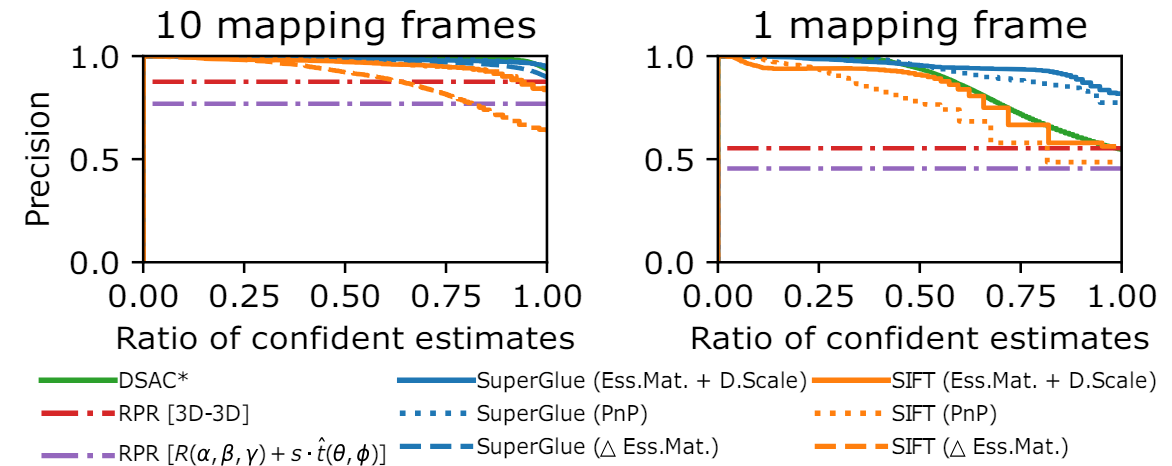
\includegraphics[width=0.6\textwidth]{pics/Proposal/partial_7scene.png}
  \caption[Hiệu quả của các mô hình khi giới hạn ảnh tham khảo]{Hiệu quả của những mô hình khi tập 7Scenes chỉ có 10/1 ảnh tham khảo, đánh giá về độ chính xác. Đối với những mô hình RPR không có phương pháp đánh giá về độ đáng tin cậy của dự đoán, một đường thẳng ngang sẽ được dùng để thể hiện độ chính xác}
\end{figure}

Để có thể phản ánh một môi trường thực tế, nơi mà ảnh tham khảo truy xuất được cách xa một khoảng đáng kể so với ảnh truy vấn, $K$ ảnh tham khảo mang nhiều thông tin nhất sẽ được chọn làm đại diện qua giải thuật gom cụm K-means.

Hai đồ thị trên thể hiện sự thay đổi về độ chính xác, những dự đoán có $VCRE<80px$ khi tỷ lệ kết quả chấp nhận thay đổi. Tỷ lệ số dự đoán chấp nhận sẽ tăng dần khi ngưỡng chấp nhận dần lỏng ra. Điều này đồng thời cũng làm cho độ chính xác cũng giảm dần do tăng khả năng những dự đoán không có cơ sở chắc chắn cũng được xem là đáng tin. Trong trường hợp này, những mô hình 2D-2D, đặc biệt là mô hình sử dụng SuperGlue, có kết quả tốt hơn so với những mô hình còn lại. Điều này thể hiện rõ nhất trong khoảng 0.5~1.0 ở cả 2 kịch bản $K=10$ và $K=1$.

Mô hình DSAC* vẫn có kết quả cạnh tranh. Tuy nhiên, phương pháp này lại quá phụ thuộc vào tập dữ liệu. Trong khi đó, những mô hình khác được huấn luyện trên tập ScanNet vẫn có kết quả tốt trên tập 7Scenes. Phương pháp sử dụng phép Triangulation cũng có kết quả cạnh tranh, tuy nhiên lại không thể hoạt động chỉ với một ảnh tham khảo. Những phương pháp Feat.Matching - Depth Scale có khả năng khái quát hóa tốt hơn những phương pháp RPR End-to-End, thể hiện qua hiệu quả tương đối tốt hơn.

\subsubsection{Tập dữ liệu Niantic}

\begin{figure}[H]
  \centering
  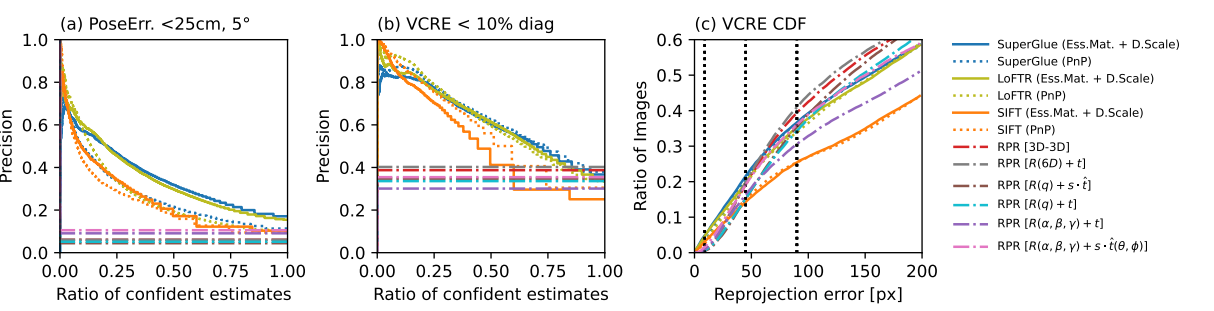
\includegraphics[width=\textwidth]{pics/Proposal/all_niantic.png}
  \caption{Hiệu quả của các mô hình trên tập dữ liệu Niantic, xác định theo độ chính xác và số ảnh có sai số phản chiếu dưới ngưỡng}
\end{figure}

Qua kết quả thu được, tập dữ liệu Niantic có độ khó cao hơn đáng kể so với tập dữ liệu 7Scenes với mọi phương pháp. Trong tập dữ liệu Niantic, những phương pháp Feat.Matching - Depth Scale tiếp tục có kết quả tốt. Tuy nhiên, ở những ngưỡng đáng tin cậy rộng hơn, những phương pháp RPR lại có kết quả tốt hơn. Điều này có thể giải thích được qua hiện tượng: khi số cặp đặc trưng tương quan là không đủ chất lượng, độ lệch đơn vị vị trí được sinh ra có sai số rất lớn so với thực tế ở những phương pháp Feat.Matching - Depth Scale. Những phương pháp RPR End-to-End cho ra kết quả tốt khi ngưỡng chính xác rộng, nhưng lại có kết quả không tốt khi cần độ chính xác cao. Ngoài ra, những phương pháp RPR End-to-End cũng không thể cung cấp độ tin cậy cho dự đoán của mô hình, không thể loại bỏ những dự đoán có khả năng sai cao.
